\documentclass[xetex,mathserif,serif,aspectratio=169]{beamer}

\usepackage{xltxtra}
\usepackage{color}
\usepackage{url}
\usepackage{listings}
\usepackage{fontspec}
\usepackage{geometry}
\usepackage{lastpage}
\usepackage{fancyhdr}
\usepackage{amsmath}
\usepackage{amsthm}
\usepackage{amssymb}
\usepackage{blkarray}
\usepackage{multicol}
\usepackage{relsize}
\usepackage{listings}
\usepackage{xunicode}
\usepackage{xltxtra}
\usepackage{color}
\usepackage{url}
\usefonttheme[onlymath]{serif}

\definecolor{solarized@base03}{HTML}{002B36}
\definecolor{solarized@base02}{HTML}{073642}
\definecolor{solarized@base01}{HTML}{586e75}
\definecolor{solarized@base00}{HTML}{657b83}
\definecolor{solarized@base0}{HTML}{839496}
\definecolor{solarized@base1}{HTML}{93a1a1}
\definecolor{solarized@base2}{HTML}{EEE8D5}
\definecolor{solarized@base3}{HTML}{FDF6E3}
\definecolor{solarized@yellow}{HTML}{B58900}
\definecolor{solarized@orange}{HTML}{CB4B16}
\definecolor{solarized@red}{HTML}{DC322F}
\definecolor{solarized@magenta}{HTML}{D33682}
\definecolor{solarized@violet}{HTML}{6C71C4}
\definecolor{solarized@blue}{HTML}{268BD2}
\definecolor{solarized@cyan}{HTML}{2AA198}
\definecolor{solarized@green}{HTML}{859900}
\definecolor{yaleblue}{HTML}{0E4C92}

\newcommand{\yellow}[1]{\textcolor{solarized@yellow}{#1}}
\newcommand{\orange}[1]{\textcolor{solarized@orange}{#1}}
\newcommand{\red}[1]{\textcolor{solarized@red}{#1}}
\newcommand{\magenta}[1]{\textcolor{solarized@magenta}{#1}}
\newcommand{\violet}[1]{\textcolor{solarized@violet}{#1}}
\newcommand{\blue}[1]{\textcolor{solarized@blue}{#1}}
\newcommand{\cyan}[1]{\textcolor{solarized@cyan}{#1}}
\newcommand{\green}[1]{\textcolor{solarized@green}{#1}}
\newcommand{\yblue}[1]{\textcolor{yaleblue}{#1}}
\newcommand{\base}[1]{\textcolor{solarized@base01}{#1}}


\defaultfontfeatures{Mapping=tex-text}
\hypersetup{pdfstartview={FitH}}

\newcommand{\old}[1]{\fontspec[Alternate=1,Ligatures={Common}]{Hoefler Text}\fontsize{18pt}{30pt}\selectfont #1}%
\newcommand{\oldA}[1]{\fontspec[Alternate=1,Ligatures={Common, Rare}]{Hoefler Text}\fontsize{12pt}{15pt}\selectfont #1}%
\newcommand{\oldB}[1]{\fontspec[Ligatures={Common}]{Didot}\fontsize{12pt}{15pt}\color{solarized@base02}\selectfont #1}%
\newcommand{\tfont}[1]{\fontspec[Alternate=1,Ligatures={Common}]{Hoefler Text}\fontsize{12pt}{20pt}\selectfont #1}%
\newcommand{\dfont}[1]{\fontspec[Ligatures={Common}]{Didot}\fontsize{12pt}{12pt}\selectfont #1}%

\setbeamerfont{title}{family=\old}
\setbeamerfont{author}{family=\tfont}%
\setbeamerfont{frametitle}{family=\oldA}
\setbeamerfont{date}{family=\dfont}

\setbeamertemplate{navigation symbols}{}
\setbeamertemplate{footline}[text line]{%
  \parbox{0.99\linewidth}{
    \normalsize\vspace*{-24pt}\hfill{\color{solarized@base00}\insertframenumber/\inserttotalframenumber}
  }
}


\setlength{\parindent}{0pt}
\setlength{\parskip}{12pt}

\setbeamercolor{structure}{bg=solarized@base3, fg=solarized@base02}
\setbeamercolor{titlelike}{fg=solarized@cyan}
\setbeamercolor{title}{fg=solarized@blue}
\setbeamercolor{subtitle}{fg=solarized@magenta}
\setbeamercolor{alerted text}{fg=orange}
\setbeamercolor{itemize}{fg=solarized@base02}
\setbeamercolor{background canvas}{bg=solarized@base3}
\setbeamercolor{enumerate subitem}{fg=solarized@base02}

\newcommand{\minimize}{\mathop{\mathrm{minimize}}}
\newcommand{\argmin}{\mathop{\mathrm{arg\,min}}}
\newcommand{\argmax}{\mathop{\mathrm{arg\,max}}}
\newcommand{\st}{\mathop{\mathrm{subject\,\,to}}}


\usepackage[]{algorithm2e}
\usepackage{../kbordermatrix}

\begin{document}

%%%%%%%%%%%%%%%%%%%%%%%%%%%%%%%%%%%%%%%%%%%%%%%%%%%
\begin{frame}[fragile] \frametitle{} \oldB \small

\vfill

{\fontsize{0.7cm}{0cm}\selectfont Lecture 18 \\\vspace{0.2cm}
Transfer Learning and Computer Vision I}\\\vspace{0.5cm}
04 April 2016

\vspace{2cm}

\begin{minipage}{0.6\textwidth}
Taylor B. Arnold \\
Yale Statistics \\
STAT 365/665
\end{minipage}
\hfill
\begin{minipage}{0.3\textwidth}\raggedleft

\includegraphics[scale=0.3]{../yale-logo.png}
\end{minipage}%

\end{frame}

%%%%%%%%%%%%%%%%%%%%%%%%%%%%%%%%%%%%%%%%%%%%%%%%%%%
\begin{frame}[fragile] \frametitle{} \oldB \small

Notes:
\begin{itemize}
\item Problem set 6 is online and due \textbf{this} Friday, April 8th
\item Problem set 7 is online and due \textbf{next} Friday, April 15th
\item No class next week
\end{itemize}

\end{frame}

%%%%%%%%%%%%%%%%%%%%%%%%%%%%%%%%%%%%%%%%%%%%%%%%%%%
\begin{frame}[fragile] \frametitle{}

\begin{flushright}
{\color{yaleblue}\sc\fontsize{1cm}{0.5cm}\selectfont Autoencoders and Transfer Learning}
\end{flushright}

\end{frame}

%%%%%%%%%%%%%%%%%%%%%%%%%%%%%%%%%%%%%%%%%%%%%%%%%%%
\begin{frame}[fragile] \frametitle{} \oldB \small

\yblue{\textbf{An Autoencoder}}

An autoencoder is a learning algorithm that attempts to
learn a compressed representation of its output. It is
conceptually an unsupervised task, but one that neural
networks are quite good at.

\end{frame}

%%%%%%%%%%%%%%%%%%%%%%%%%%%%%%%%%%%%%%%%%%%%%%%%%%%
\begin{frame}[fragile] \frametitle{} \oldB \small

\yblue{\textbf{Neural network Autoencoder}}

To build a neural network auto-encoder, we simply build a neural
network where the input is equal to the output. This is only meaningful
when there exists a hidden layer with fewer nodes than the input
layer (otherwise we can perfectly reconstruct the image):

\begin{center}
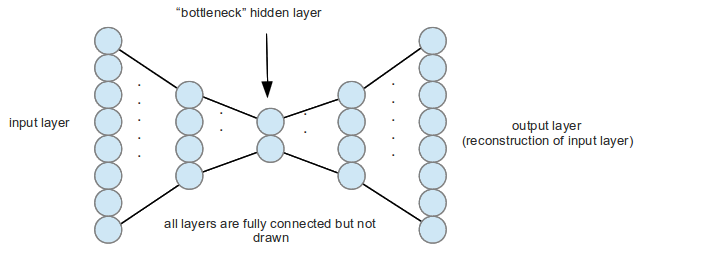
\includegraphics[height=0.5\textheight]{img/autoencoder_network1.png}
\end{center}

\end{frame}

%%%%%%%%%%%%%%%%%%%%%%%%%%%%%%%%%%%%%%%%%%%%%%%%%%%
\begin{frame}[fragile] \frametitle{} \oldB \small

\yblue{\textbf{The botteneck layer}}

Notice that by storing the values in the hidden layer with
the fewest nodes, we get a compression of the input into a
lower dimensional space (other hidden layers also do this, but
may do a smaller amount of compression).

\end{frame}

%%%%%%%%%%%%%%%%%%%%%%%%%%%%%%%%%%%%%%%%%%%%%%%%%%%
\begin{frame}[fragile] \frametitle{} \oldB \small

\yblue{\textbf{Dimensionality reduction}}

We can reason that for many tasks, if this lower dimensional representation
does a good job of reconstructing the image, there is enough information
contained in that layer to also do learning tasks. If the degree of compression
is high, this can aid in learning because the input dimensionality has been
reduced.

\pause This is exactly the same as computing principal components and then using
the first few components to do regression on.

\pause It turns out, very helpfully, that the hidden layers of non-autoencoding
networks perform a supervised dimensionality reduction. We can often think of
the inner layers in the same way as the bottleneck layers for an autoencoder.

\end{frame}

%%%%%%%%%%%%%%%%%%%%%%%%%%%%%%%%%%%%%%%%%%%%%%%%%%%
\begin{frame}[fragile] \frametitle{} \oldB \small

\yblue{\textbf{Autoencoder demo}}

A live demo of an autoencoder on the MNIST-10 dataset:
\begin{quote}
\url{http://cs.stanford.edu/people/karpathy/convnetjs/demo/autoencoder.html}
\end{quote}

\end{frame}


%%%%%%%%%%%%%%%%%%%%%%%%%%%%%%%%%%%%%%%%%%%%%%%%%%%
\begin{frame}[fragile] \frametitle{} \oldB \footnotesize

\yblue{\textbf{Transfer learning}}

Remember when we were predicting crimes on the City of Chicago dataset; many
of you were quite concerned about why the following worked so well:
\begin{enumerate}
\item Train a model on the output $Z$, using the covariate matrix $X$
\item Use the predicted values, along with $X$, to learn a new output $Y$
\end{enumerate}
\pause We can do this with neural networks in a more natural way by:
\begin{enumerate}
\item Train a neural network on an output $Z$, using the inputs $X$
\item Remove the learned output layer from this network, and attach another
output layer to capture a new output $Y$
\item Train this new model, either using the weights from the first step as
a starting point (pre-training) or freezing them (transfer learning)
\end{enumerate}
Does this process make more intuitive sense now that we can see the first
step as supervised dimensionality reduction?

\end{frame}

%%%%%%%%%%%%%%%%%%%%%%%%%%%%%%%%%%%%%%%%%%%%%%%%%%%
\begin{frame}[fragile] \frametitle{} \oldB \footnotesize

\yblue{\textbf{Why is this all important?}}

In order to get state-of-the-art results using neural networks, we
need to train very large and deep models. This requires a lot of
data and computing power, both of which most users do not have.
To circumvent this, some combination of pre-training or transfer
learning is used instead.

This is largely why understanding the recent history of computer
vision models is so important; most computer visions tasks will
require one to use and modify these models in some form.

\end{frame}

%%%%%%%%%%%%%%%%%%%%%%%%%%%%%%%%%%%%%%%%%%%%%%%%%%%
\begin{frame}[fragile] \frametitle{} \oldB \small

\yblue{\textbf{Autoencoding, Transfer Learning, and Pre-training}}

Good references for these topics are given by
\begin{quote}
Mesnil, G., Dauphin, Y., Glorot, X., Rifai, S., Bengio, Y., Goodfellow, I., Lavoie, E., Muller, X., Desjardins, G., Warde-Farley, D., Vincent, P., Courville, A., and Bergstra, J. (2011). Unsupervised and transfer learning challenge: a deep learning approach.
\end{quote}
And,
\begin{quote}
Long, Jonathan L., Ning Zhang, and Trevor Darrell. "Do Convnets Learn Correspondence?." Advances in Neural Information Processing Systems. 2014.
\end{quote}

\end{frame}



%%%%%%%%%%%%%%%%%%%%%%%%%%%%%%%%%%%%%%%%%%%%%%%%%%%
\begin{frame}[fragile] \frametitle{}

\begin{flushright}
{\color{yaleblue}\sc\fontsize{1cm}{1cm}\selectfont Computer Vision I}
\end{flushright}

\end{frame}

%%%%%%%%%%%%%%%%%%%%%%%%%%%%%%%%%%%%%%%%%%%%%%%%%%%
\begin{frame}[fragile] \frametitle{} \oldB \small

\yblue{\textbf{CNN Review}}

A 5x5 kernel with a stride of $1$:

\begin{center}
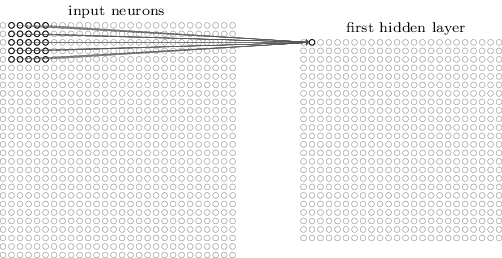
\includegraphics[height=0.66\textheight]{img/tikz45.png}
\end{center}

\end{frame}

%%%%%%%%%%%%%%%%%%%%%%%%%%%%%%%%%%%%%%%%%%%%%%%%%%%
\begin{frame}[fragile] \frametitle{} \oldB \small

\yblue{\textbf{CNN Review}}

Max pooling with 2x2 kernel and stride of $2$:

\begin{center}
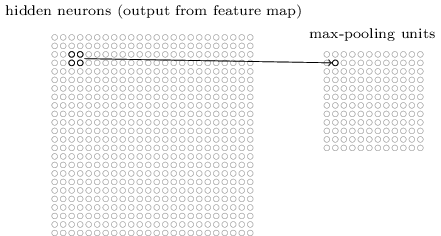
\includegraphics[height=0.66\textheight]{img/tikz47.png}
\end{center}

\end{frame}

%%%%%%%%%%%%%%%%%%%%%%%%%%%%%%%%%%%%%%%%%%%%%%%%%%%
\begin{frame}[fragile] \frametitle{} \oldB \small

\yblue{\textbf{CNN Review}}

A complete CNN model:

\begin{center}
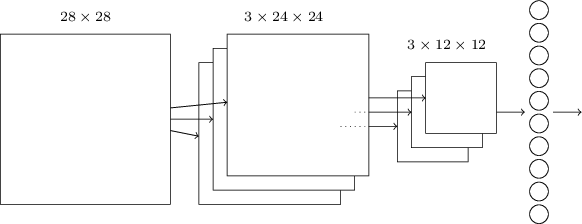
\includegraphics[height=0.5\textheight]{img/tikz49.png}
\end{center}

\end{frame}


%%%%%%%%%%%%%%%%%%%%%%%%%%%%%%%%%%%%%%%%%%%%%%%%%%%
\begin{frame}[fragile] \frametitle{} \oldB \footnotesize

\yblue{\textbf{Convolutional Models in Computer Vision}}

There is a long history of specific advances and uses of convolutional
neural networks. Today, I'll focus on the following set of models: \vspace*{-0.5cm}
\begin{itemize}
\item LeNet-5 (1998)
\item AlexNet (2012)
\item OverFeat (2013)
\item VGG-16, VGG-19 (2014)
\item GoogLeNet (2014)
\item PReLUnet (2015)
\item ResNet-50, ResNet-101, ResNet-152 (2015)
\item SqueezeNet (2016)
\item Stochastic Depth (2016)
\item ResNet-200, ResNet-1001 (2016)
\end{itemize} \vspace*{-0.5cm}
When you hear about these models people may be referring to: the architecture,
the architecture and weights, or just to the general approach.

\end{frame}

%%%%%%%%%%%%%%%%%%%%%%%%%%%%%%%%%%%%%%%%%%%%%%%%%%%
\begin{frame}[fragile] \frametitle{} \oldB \small

\yblue{\textbf{LeNet-5 (1998)}}

LeNet was one of first models to really show the power of convolutional
neural networks. It was first applied to the MNIST-10 dataset, created
by a similar group of individuals:
\begin{quote}
LeCun, Y., Bottou, L., Bengio, Y. and Haffner, P., 1998. Gradient-based
learning applied to document recognition. Proceedings of the IEEE, 86(11),
pp.2278-2324.
\end{quote}

\end{frame}

%%%%%%%%%%%%%%%%%%%%%%%%%%%%%%%%%%%%%%%%%%%%%%%%%%%
\begin{frame}[fragile] \frametitle{} \oldB \small

\begin{center}
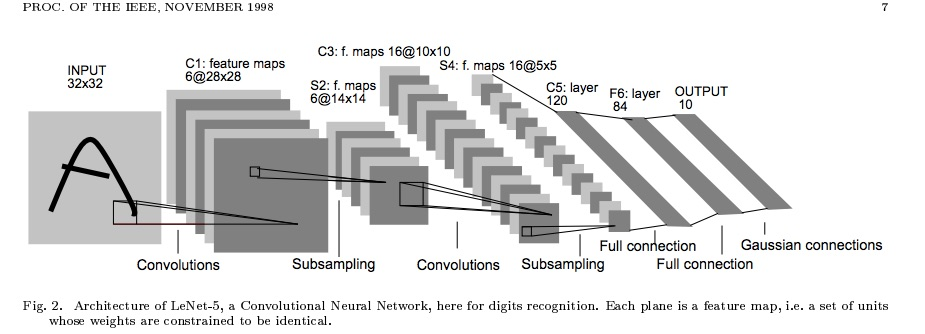
\includegraphics[width=\textwidth]{img/lenet5.jpg}
\end{center}

\end{frame}

%%%%%%%%%%%%%%%%%%%%%%%%%%%%%%%%%%%%%%%%%%%%%%%%%%%
\begin{frame}[fragile] \frametitle{} \oldB \small

\begin{center}
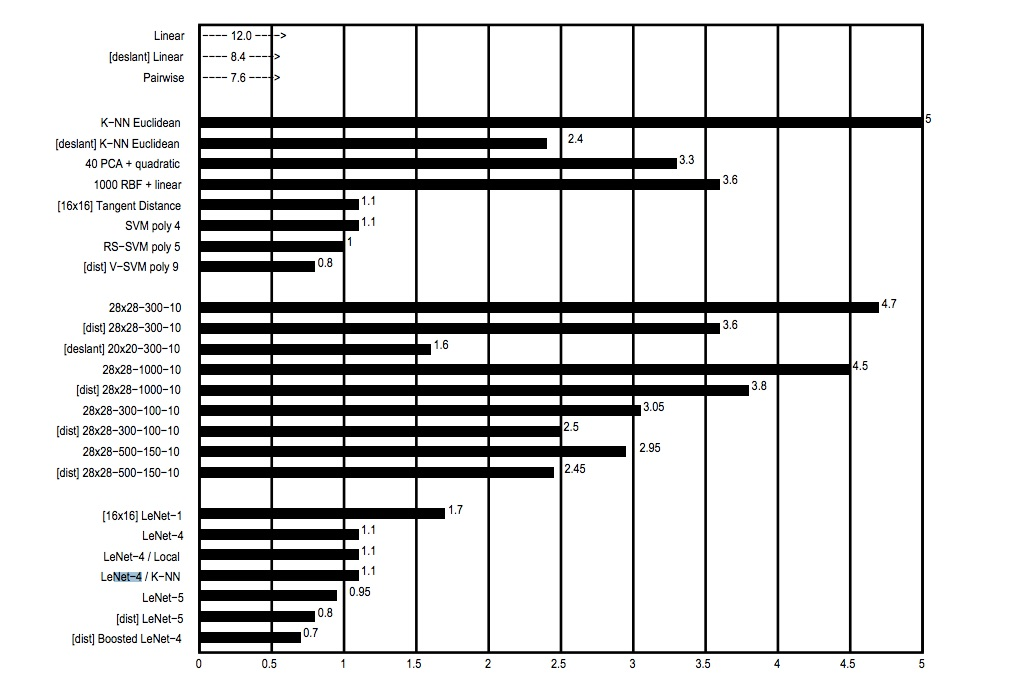
\includegraphics[width=0.7\textwidth]{img/leNetCompare.jpg}
\end{center}

\end{frame}

%%%%%%%%%%%%%%%%%%%%%%%%%%%%%%%%%%%%%%%%%%%%%%%%%%%
\begin{frame}[fragile] \frametitle{} \oldB \small

\textbf{\magenta{Python demo I: LeNet-5 for MNIST10}}

\end{frame}

%%%%%%%%%%%%%%%%%%%%%%%%%%%%%%%%%%%%%%%%%%%%%%%%%%%
\begin{frame}[fragile] \frametitle{} \oldB \small

\textbf{\magenta{Python demo II:  LeNet-5 with ``Distortions" (i.e., Data augmentation)}}

\end{frame}

%%%%%%%%%%%%%%%%%%%%%%%%%%%%%%%%%%%%%%%%%%%%%%%%%%%
\begin{frame}[fragile] \frametitle{} \oldB \small

\begin{center}
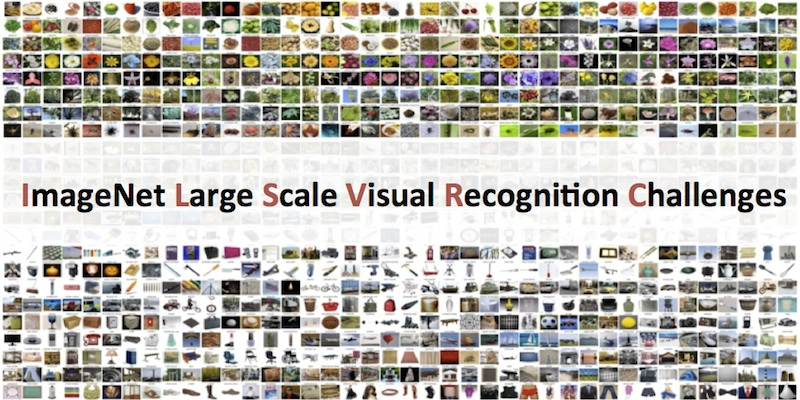
\includegraphics[width=\textwidth]{img/ilsvrc.jpg}
\end{center}

\end{frame}

%%%%%%%%%%%%%%%%%%%%%%%%%%%%%%%%%%%%%%%%%%%%%%%%%%%
\begin{frame}[fragile] \frametitle{} \oldB \small

\yblue{\textbf{ImageNet Overview (through 2014)}}

An excellent summery paper of the ILSVCR challeneg, that
describes in more detail than I will here, is given by:
\begin{quote}
Olga Russakovsky, et al. "ImageNet Large Scale Visual Recognition Challenge".
arXiv preprint arXiv:1409.0575v3 (2015).
\end{quote}

\end{frame}

%%%%%%%%%%%%%%%%%%%%%%%%%%%%%%%%%%%%%%%%%%%%%%%%%%%
\begin{frame}[fragile] \frametitle{} \oldB \small

\begin{center}
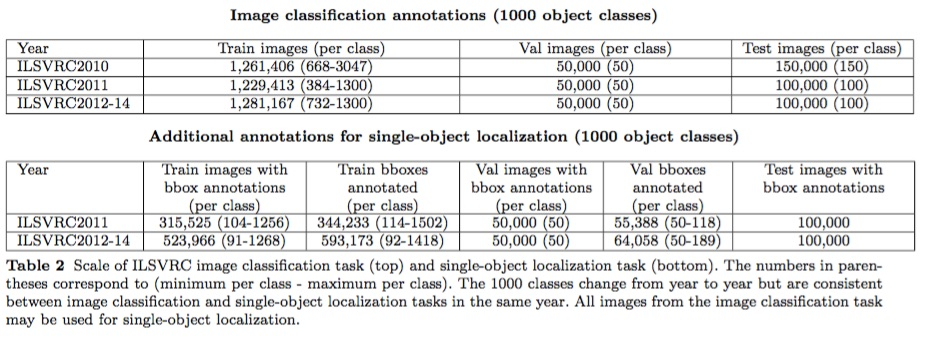
\includegraphics[width=\textwidth]{img/ilsvrcSize.jpg}
\end{center}

\end{frame}


%%%%%%%%%%%%%%%%%%%%%%%%%%%%%%%%%%%%%%%%%%%%%%%%%%%
\begin{frame}[fragile] \frametitle{} \oldB \small

\begin{center}
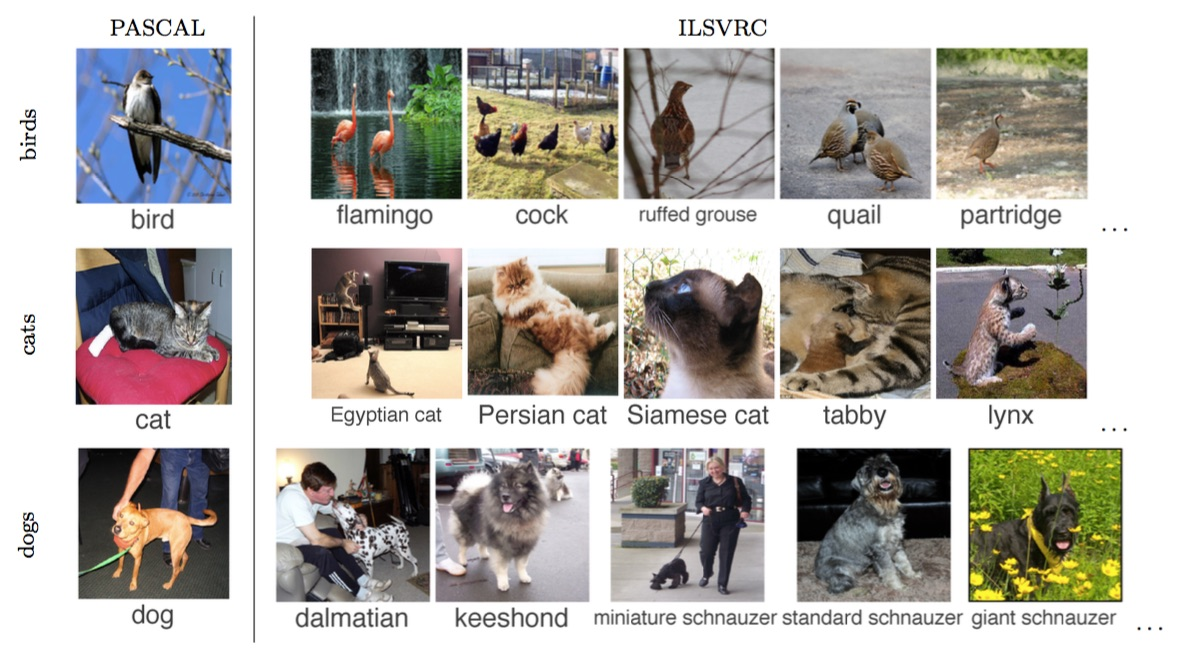
\includegraphics[width=\textwidth]{img/ilsvrcCategories.jpg}
\end{center}

\end{frame}


%%%%%%%%%%%%%%%%%%%%%%%%%%%%%%%%%%%%%%%%%%%%%%%%%%%
\begin{frame}[fragile] \frametitle{} \oldB \small

\begin{center}
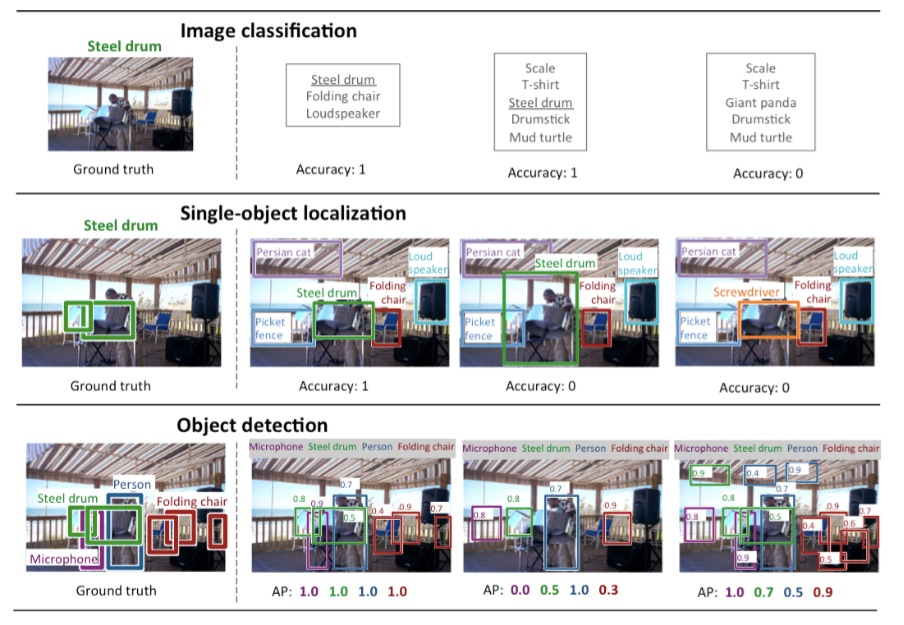
\includegraphics[width=0.85\textwidth]{img/ilsvrcTasks.jpg}
\end{center}

\end{frame}


%%%%%%%%%%%%%%%%%%%%%%%%%%%%%%%%%%%%%%%%%%%%%%%%%%%
\begin{frame}[fragile] \frametitle{} \oldB \small

\begin{center}
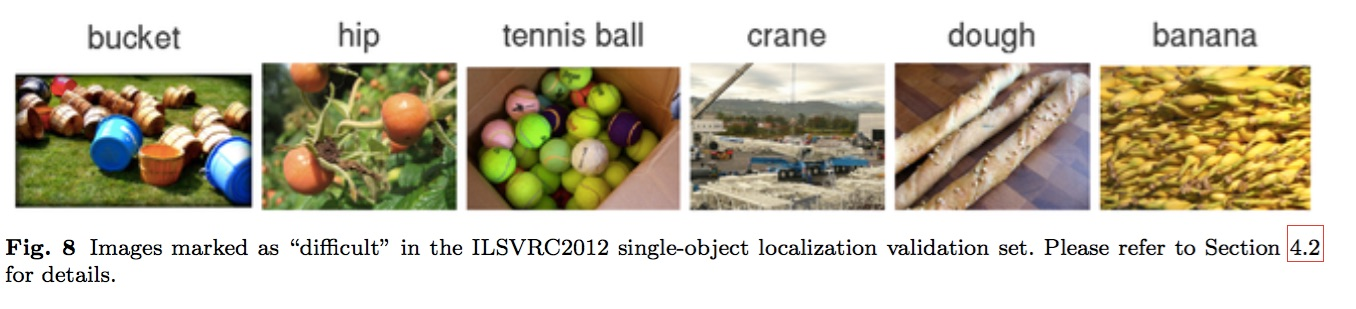
\includegraphics[width=\textwidth]{img/ilsvrcDifficult.jpg}
\end{center}

\end{frame}


%%%%%%%%%%%%%%%%%%%%%%%%%%%%%%%%%%%%%%%%%%%%%%%%%%%
\begin{frame}[fragile] \frametitle{} \oldB \small

\begin{center}
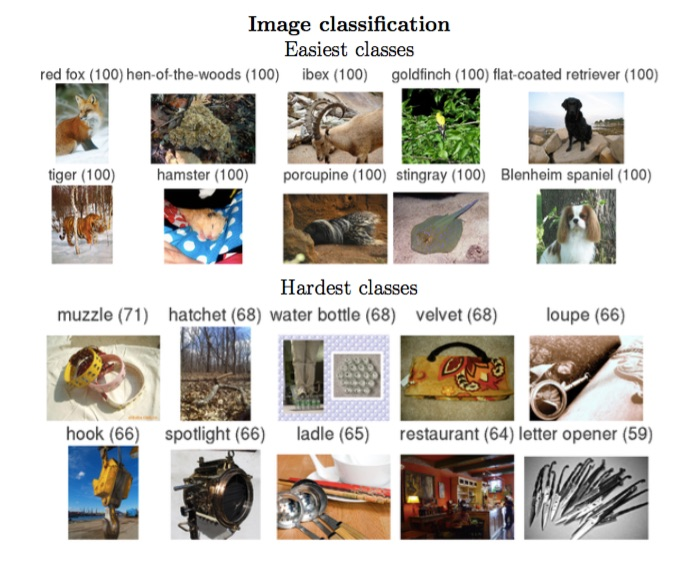
\includegraphics[width=0.7\textwidth]{img/ilsvrcDifficultClasses.jpg}
\end{center}

\end{frame}


%%%%%%%%%%%%%%%%%%%%%%%%%%%%%%%%%%%%%%%%%%%%%%%%%%%
\begin{frame}[fragile] \frametitle{} \oldB \small

\begin{center}
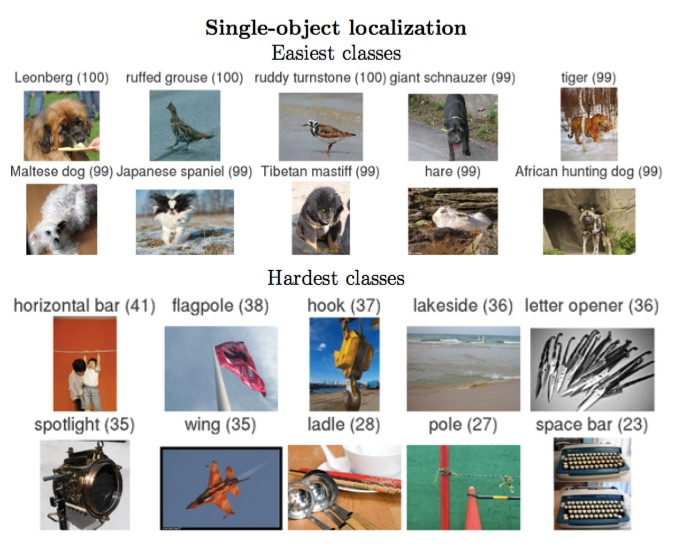
\includegraphics[width=0.7\textwidth]{img/ilsvrcDifficultLocalization.jpg}
\end{center}

\end{frame}


%%%%%%%%%%%%%%%%%%%%%%%%%%%%%%%%%%%%%%%%%%%%%%%%%%%
\begin{frame}[fragile] \frametitle{} \oldB \small

\begin{center}
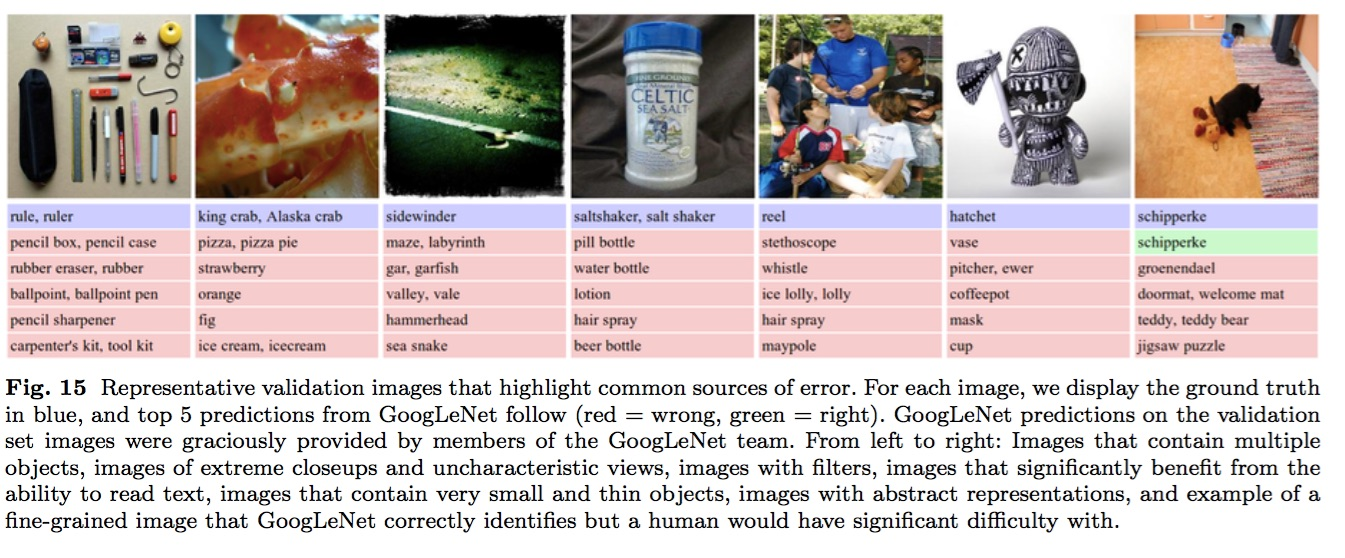
\includegraphics[width=\textwidth]{img/ilsvrcCommonErrors.jpg}
\end{center}

\end{frame}


%%%%%%%%%%%%%%%%%%%%%%%%%%%%%%%%%%%%%%%%%%%%%%%%%%%
\begin{frame}[fragile] \frametitle{} \oldB \small

\begin{center}
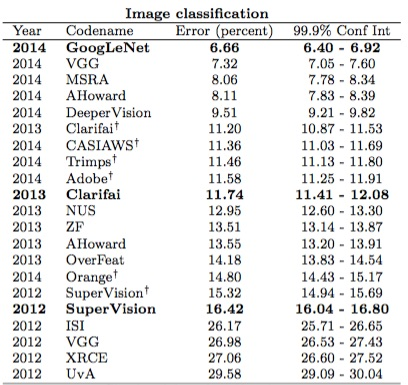
\includegraphics[width=0.63\textwidth]{img/ilsvrcClassRates.jpg}
\end{center}

\end{frame}


%%%%%%%%%%%%%%%%%%%%%%%%%%%%%%%%%%%%%%%%%%%%%%%%%%%
\begin{frame}[fragile] \frametitle{} \oldB \small

\begin{center}
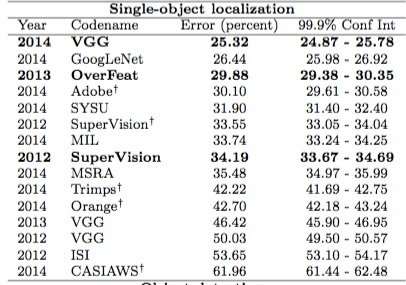
\includegraphics[width=0.7\textwidth]{img/ilsvrcLocalRates.jpg}
\end{center}

\end{frame}

%%%%%%%%%%%%%%%%%%%%%%%%%%%%%%%%%%%%%%%%%%%%%%%%%%%
\begin{frame}[fragile] \frametitle{} \oldB \small

\yblue{\textbf{AlexNet (2012)}}

A model out of the University of Toronto, now known as AlexNet,
became the first CNN to produce state-of-the-art classification
rates on the ILSVRC-2012 dataset:
\begin{quote}
Krizhevsky, Alex, Ilya Sutskever, and Geoffrey E. Hinton. "Imagenet classification with deep convolutional neural networks." In Advances in neural information processing systems, pp. 1097-1105. 2012.
\end{quote}

\end{frame}

%%%%%%%%%%%%%%%%%%%%%%%%%%%%%%%%%%%%%%%%%%%%%%%%%%%
\begin{frame}[fragile] \frametitle{} \oldB \small

\yblue{\textbf{AlexNet contributions }}

AlexNet was the first to put together several key advances, all
of which we have already used in this class:
\begin{enumerate}
\item relu units
\item multiple GPUs
\item dropout
\item data augmentation
\end{enumerate}
While not all invented by the AlexNet group, they were the first
to put them all together and figure out how to train a deep
neural network.

\end{frame}

%%%%%%%%%%%%%%%%%%%%%%%%%%%%%%%%%%%%%%%%%%%%%%%%%%%
\begin{frame}[fragile] \frametitle{} \oldB \small

\begin{center}
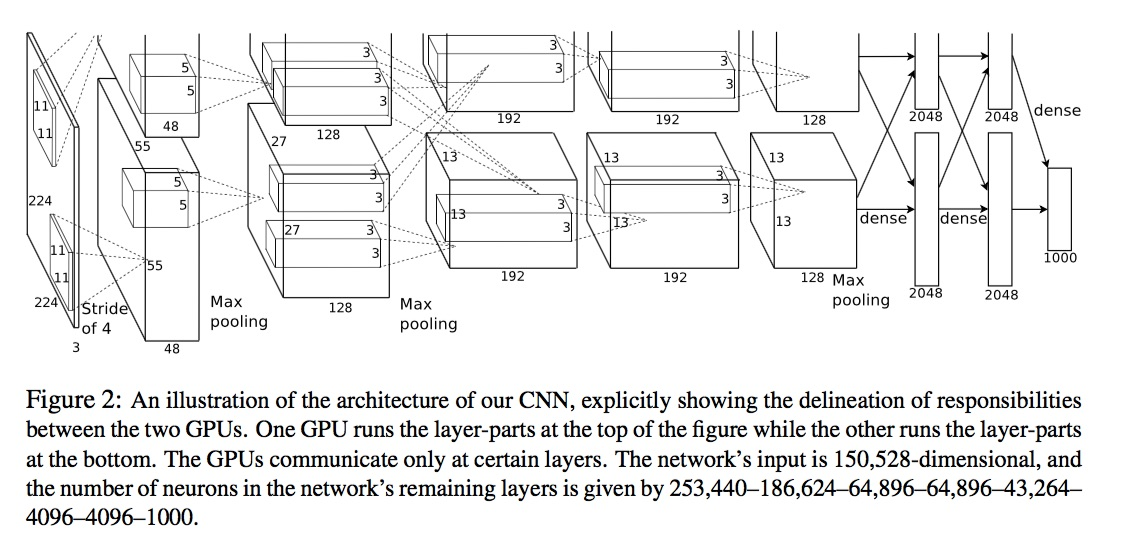
\includegraphics[width=\textwidth]{img/alexNet.jpg}
\end{center}

\end{frame}

%%%%%%%%%%%%%%%%%%%%%%%%%%%%%%%%%%%%%%%%%%%%%%%%%%%
\begin{frame}[fragile] \frametitle{} \oldB \small

\yblue{\textbf{Visualizing CNNs (2013)}}

Following the success of AlexNet, the year 2013 saw a much
larger number of neural network entrants into the ILSVRC
competition. The winning entry came about due to the
visualization techniques described in the following paper:
\begin{quote}
Zeiler, Matthew D., and Rob Fergus. "Visualizing and understanding convolutional networks." Computer vision–ECCV 2014. Springer International Publishing, 2014. 818-833.
\end{quote}
Their incredibly diverse set of techniques allowed the team
to tweak the AlexNet architecture to get even better results.

\end{frame}

%%%%%%%%%%%%%%%%%%%%%%%%%%%%%%%%%%%%%%%%%%%%%%%%%%%
\begin{frame}[fragile] \frametitle{} \oldB \small

\begin{center}
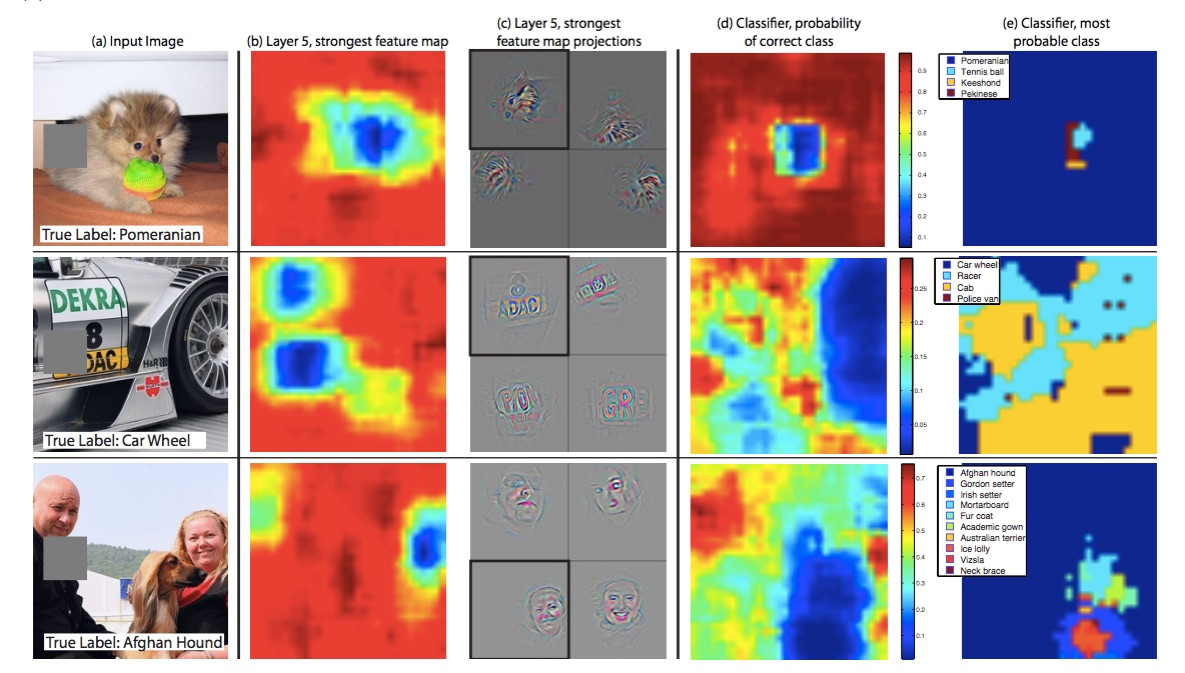
\includegraphics[width=\textwidth]{img/vizCover.jpg}
\end{center}

\end{frame}

%%%%%%%%%%%%%%%%%%%%%%%%%%%%%%%%%%%%%%%%%%%%%%%%%%%
\begin{frame}[fragile] \frametitle{} \oldB \small

\begin{center}
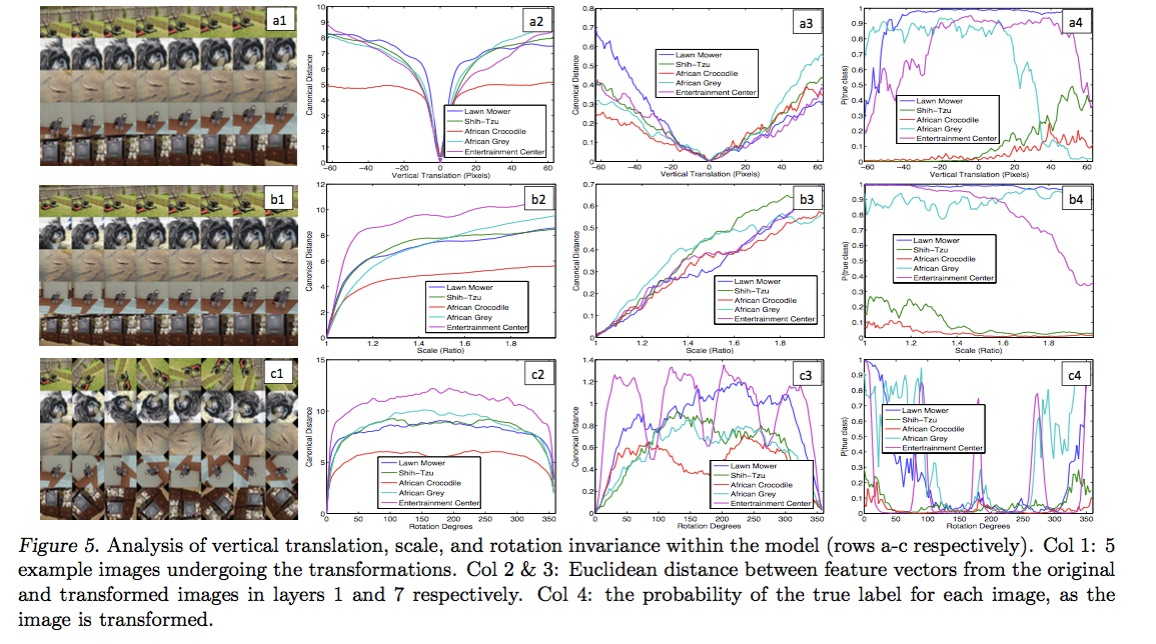
\includegraphics[width=\textwidth]{img/vizDistort.jpg}
\end{center}

\end{frame}

%%%%%%%%%%%%%%%%%%%%%%%%%%%%%%%%%%%%%%%%%%%%%%%%%%%
\begin{frame}[fragile] \frametitle{} \oldB \small

\begin{center}
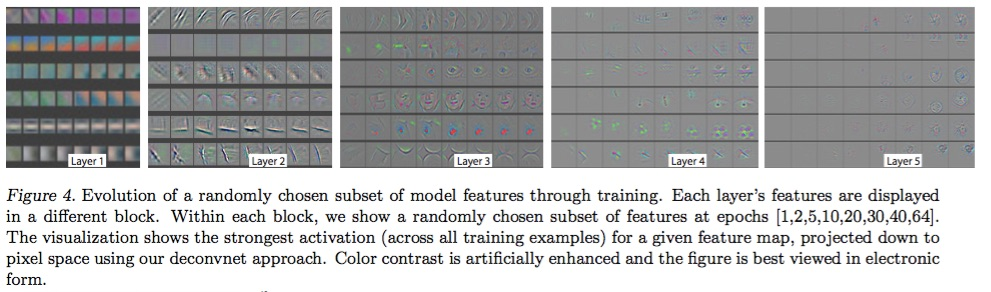
\includegraphics[width=\textwidth]{img/vizEvolve.jpg}
\end{center}

\end{frame}

%%%%%%%%%%%%%%%%%%%%%%%%%%%%%%%%%%%%%%%%%%%%%%%%%%%
\begin{frame}[fragile] \frametitle{} \oldB \small

\begin{center}
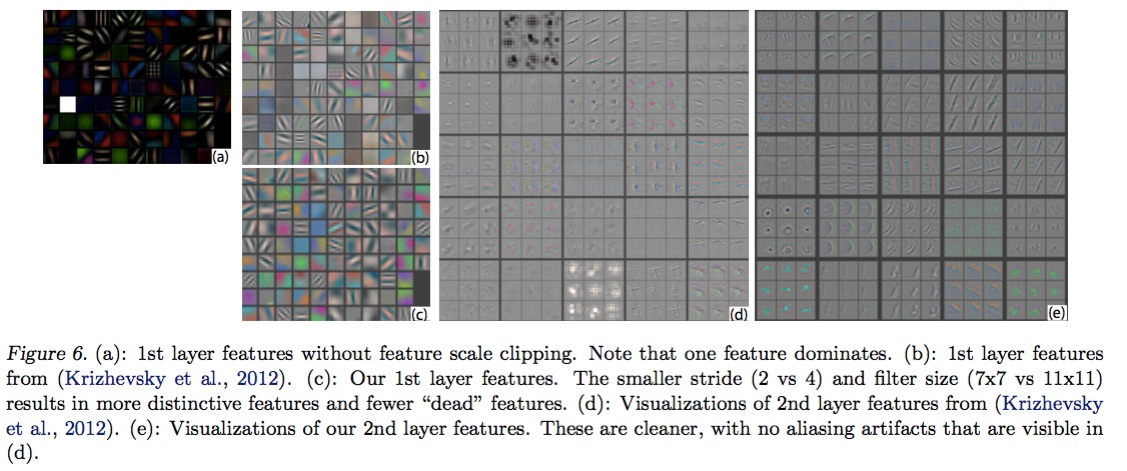
\includegraphics[width=\textwidth]{img/vizFeatureClip.jpg}
\end{center}

\end{frame}

%%%%%%%%%%%%%%%%%%%%%%%%%%%%%%%%%%%%%%%%%%%%%%%%%%%
\begin{frame}[fragile] \frametitle{} \oldB \small

\begin{center}
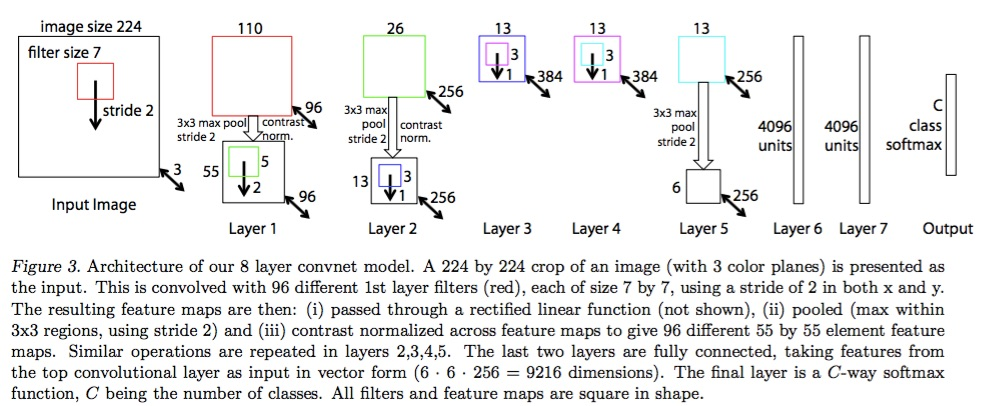
\includegraphics[width=\textwidth]{img/vizModel.jpg}
\end{center}

\end{frame}

%%%%%%%%%%%%%%%%%%%%%%%%%%%%%%%%%%%%%%%%%%%%%%%%%%%
\begin{frame}[fragile] \frametitle{} \oldB \small

A demo of applying these techniques to the MNIST dataset with ConvNetJS:

\begin{center}
\url{http://cs.stanford.edu/people/karpathy/convnetjs/demo/mnist.html}
\end{center}

\end{frame}

%%%%%%%%%%%%%%%%%%%%%%%%%%%%%%%%%%%%%%%%%%%%%%%%%%%
\begin{frame}[fragile] \frametitle{} \oldB \small

\yblue{\textbf{OverFeat (2013)}}

The 2013 competition also brought about the incredibly influential
OverFeat model from a team based at NYU:
\begin{quote}
Sermanet, Pierre, David Eigen, Xiang Zhang, Michaël Mathieu, Rob Fergus, and Yann LeCun. "Overfeat: Integrated recognition, localization and detection using convolutional networks." arXiv preprint arXiv:1312.6229 (2013).
\end{quote}
The won the image localization task, by trying to solve localization
and identification in a unified process. I'll give a very simplified
version of what they did (the paper is a great read, and I suggest
working through it if you are interested in computer vision).

\end{frame}

%%%%%%%%%%%%%%%%%%%%%%%%%%%%%%%%%%%%%%%%%%%%%%%%%%%
\begin{frame}[fragile] \frametitle{} \oldB \small

\begin{center}
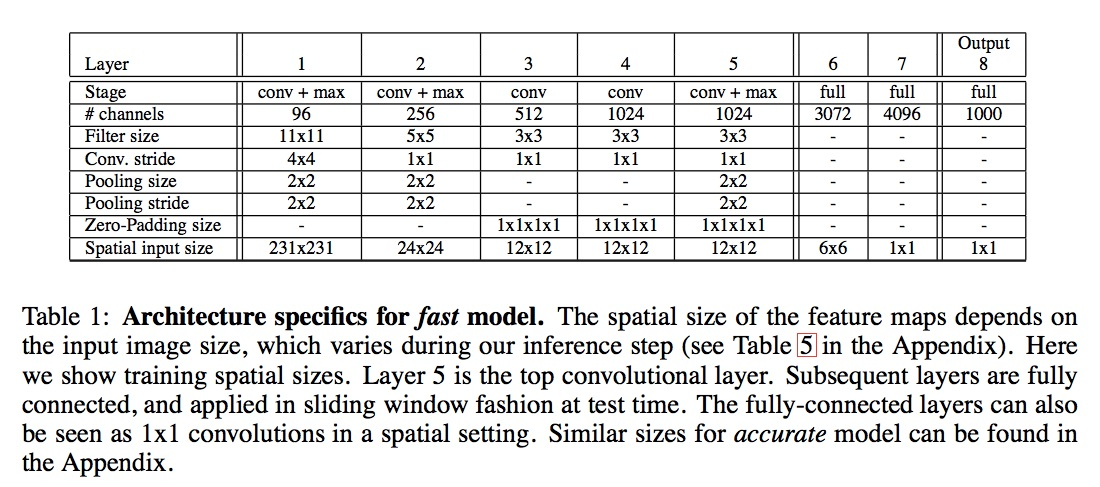
\includegraphics[width=\textwidth]{img/overFeatModel.jpg}
\end{center}

\end{frame}

%%%%%%%%%%%%%%%%%%%%%%%%%%%%%%%%%%%%%%%%%%%%%%%%%%%
\begin{frame}[fragile] \frametitle{} \oldB \small

\begin{center}
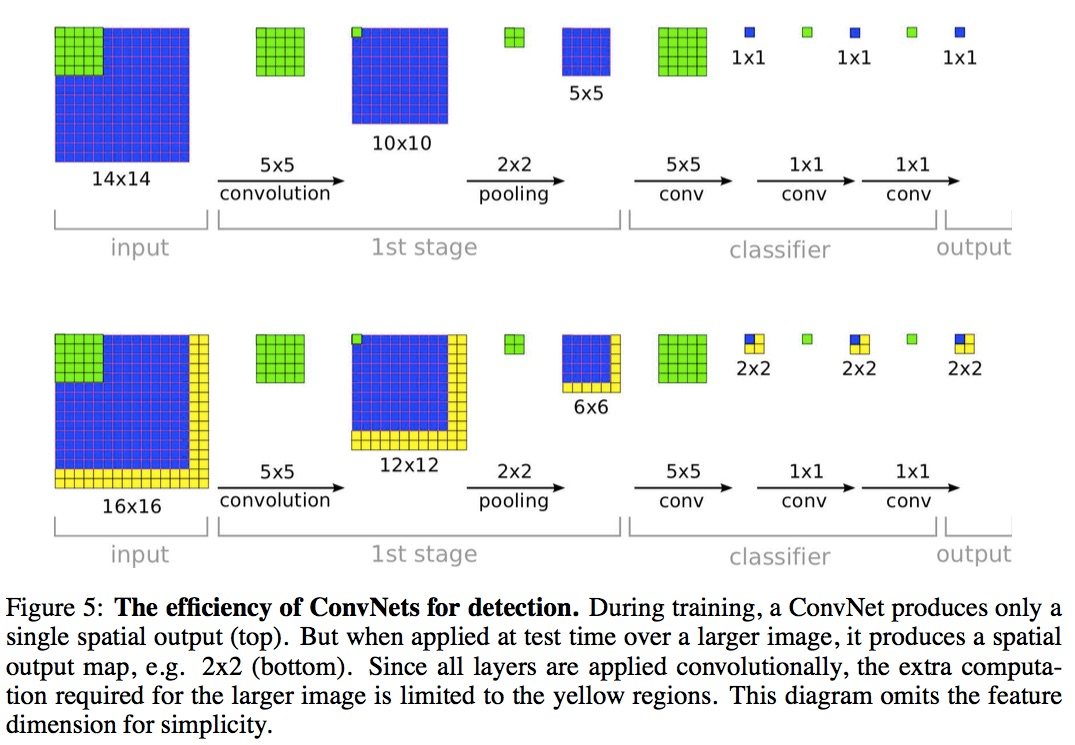
\includegraphics[width=0.75\textwidth]{img/overFeatIdea.jpg}
\end{center}

\end{frame}

%%%%%%%%%%%%%%%%%%%%%%%%%%%%%%%%%%%%%%%%%%%%%%%%%%%
\begin{frame}[fragile] \frametitle{} \oldB \small

\begin{center}
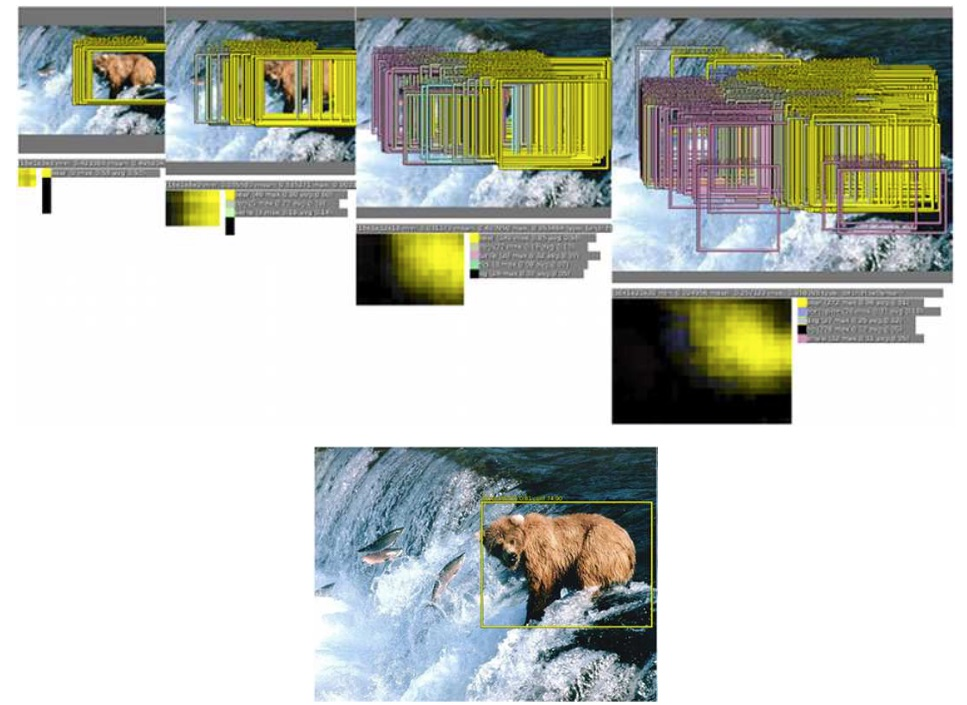
\includegraphics[width=0.8\textwidth]{img/overFeatLocal.jpg}
\end{center}

\end{frame}

%%%%%%%%%%%%%%%%%%%%%%%%%%%%%%%%%%%%%%%%%%%%%%%%%%%
\begin{frame}[fragile] \frametitle{} \oldB \small

\begin{center}
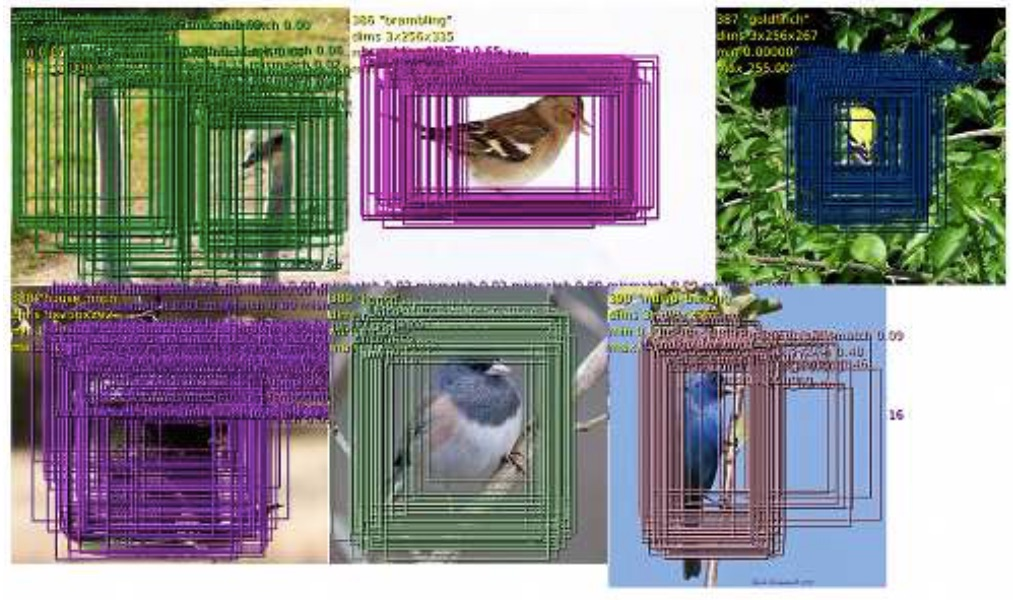
\includegraphics[width=0.95\textwidth]{img/overFeatLocalMore.jpg}
\end{center}

\end{frame}

%%%%%%%%%%%%%%%%%%%%%%%%%%%%%%%%%%%%%%%%%%%%%%%%%%%
\begin{frame}[fragile] \frametitle{} \oldB \small

\textbf{\magenta{Python demo III:  OverFeat adaptation of AlexNet (2012)}}

\end{frame}

%%%%%%%%%%%%%%%%%%%%%%%%%%%%%%%%%%%%%%%%%%%%%%%%%%%
\begin{frame}[fragile] \frametitle{} \oldB \small

\yblue{\textbf{VGG-16, VGG-19 (2014)}}

One of the top entries from 2014, by an Oxford-based team, took
advantage of significantly deeper models.
\begin{quote}
Simonyan, Karen, and Andrew Zisserman. "Very deep convolutional networks for large-scale image recognition." arXiv preprint arXiv:1409.1556 (2014).
\end{quote}

\end{frame}

%%%%%%%%%%%%%%%%%%%%%%%%%%%%%%%%%%%%%%%%%%%%%%%%%%%
\begin{frame}[fragile] \frametitle{} \oldB \small

\begin{center}
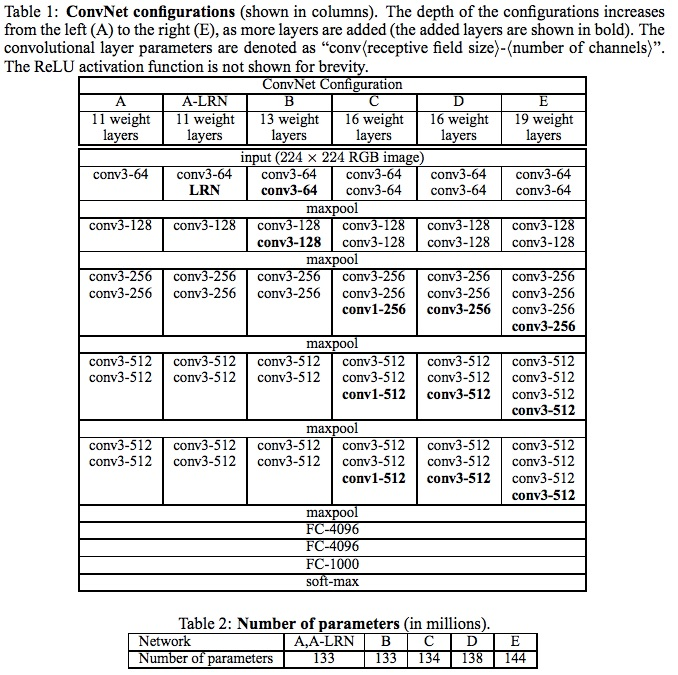
\includegraphics[width=0.5\textwidth]{img/vggModel.jpg}
\end{center}

\end{frame}

%%%%%%%%%%%%%%%%%%%%%%%%%%%%%%%%%%%%%%%%%%%%%%%%%%%
\begin{frame}[fragile] \frametitle{} \oldB \small

\textbf{\magenta{Python demo IV: Pre-trained VGG-19 Model}}

\end{frame}

%%%%%%%%%%%%%%%%%%%%%%%%%%%%%%%%%%%%%%%%%%%%%%%%%%%
\begin{frame}[fragile] \frametitle{} \oldB \small

\yblue{\textbf{GoogLeNet (2014)}}

The winning entry from 2014, by Google, also took advantage
of much deeper architectures:
\begin{quote}
Szegedy, Christian, Wei Liu, Yangqing Jia, Pierre Sermanet, Scott Reed, Dragomir Anguelov, Dumitru Erhan, Vincent Vanhoucke, and Andrew Rabinovich. "Going deeper with convolutions." In Proceedings of the IEEE Conference on Computer Vision and Pattern Recognition, pp. 1-9. 2015.
\end{quote}
They called their model GoogLeNet in honor of the original LeNet
architecture.

\end{frame}

%%%%%%%%%%%%%%%%%%%%%%%%%%%%%%%%%%%%%%%%%%%%%%%%%%%
\begin{frame}[fragile] \frametitle{} \oldB \small

\begin{center}
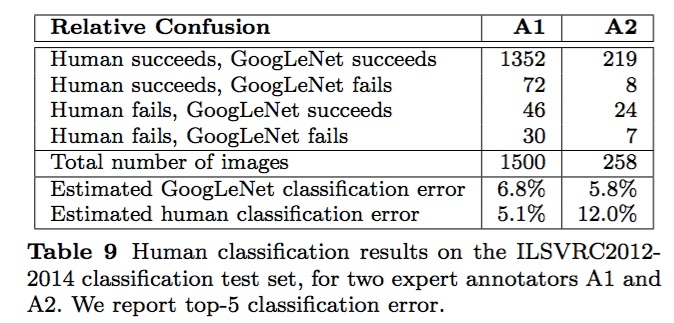
\includegraphics[width=0.8\textwidth]{img/googLeNetVsHuman.jpg}
\end{center}

\end{frame}

%%%%%%%%%%%%%%%%%%%%%%%%%%%%%%%%%%%%%%%%%%%%%%%%%%%
\begin{frame}[fragile] \frametitle{} \oldB \small

\begin{center}
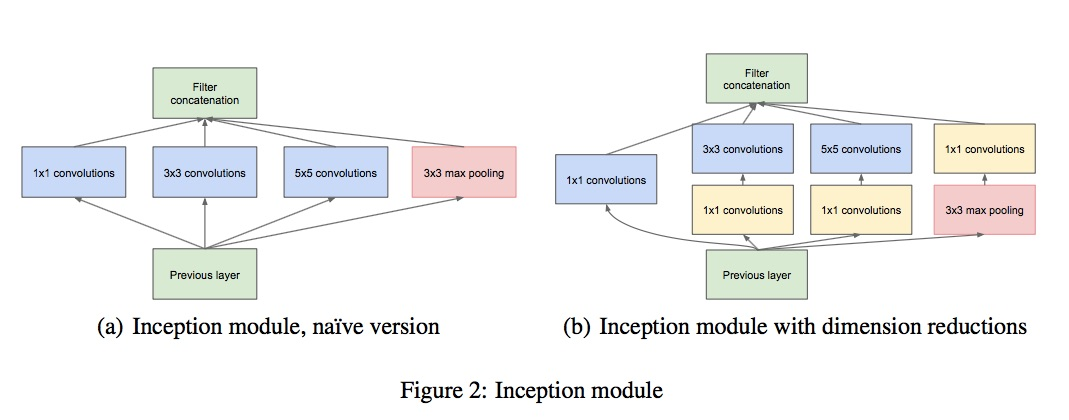
\includegraphics[width=\textwidth]{img/googLeNetInception.jpg}
\end{center}

\end{frame}

%%%%%%%%%%%%%%%%%%%%%%%%%%%%%%%%%%%%%%%%%%%%%%%%%%%
\begin{frame}[fragile] \frametitle{} \oldB \small

\begin{center}
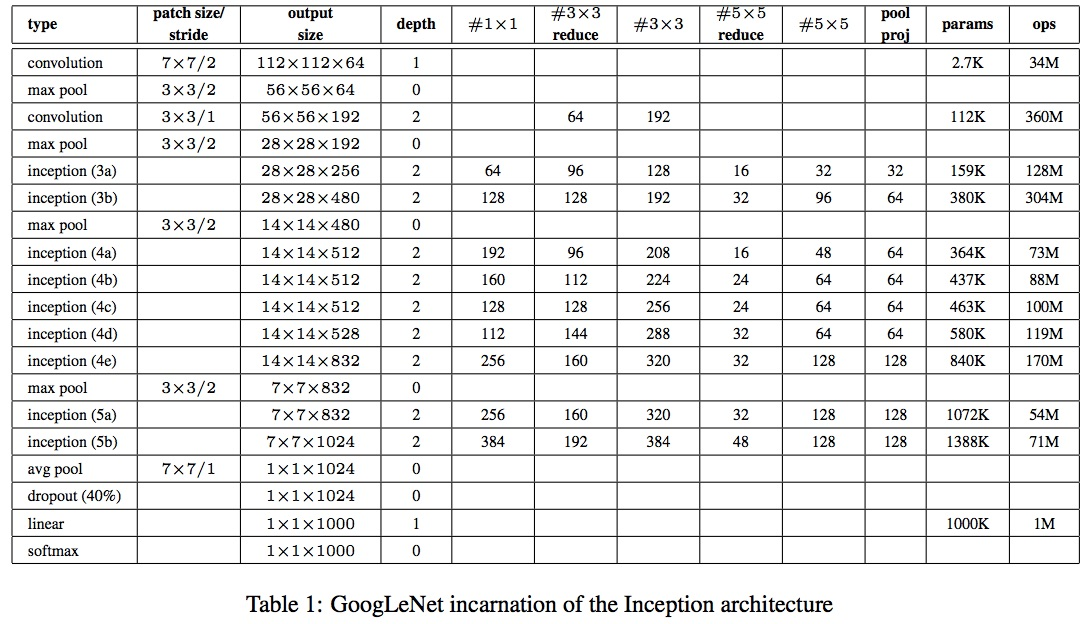
\includegraphics[width=0.95\textwidth]{img/googLeNetModel.jpg}
\end{center}

\end{frame}

%%%%%%%%%%%%%%%%%%%%%%%%%%%%%%%%%%%%%%%%%%%%%%%%%%%
\begin{frame}[fragile] \frametitle{} \oldB \small

\begin{center}
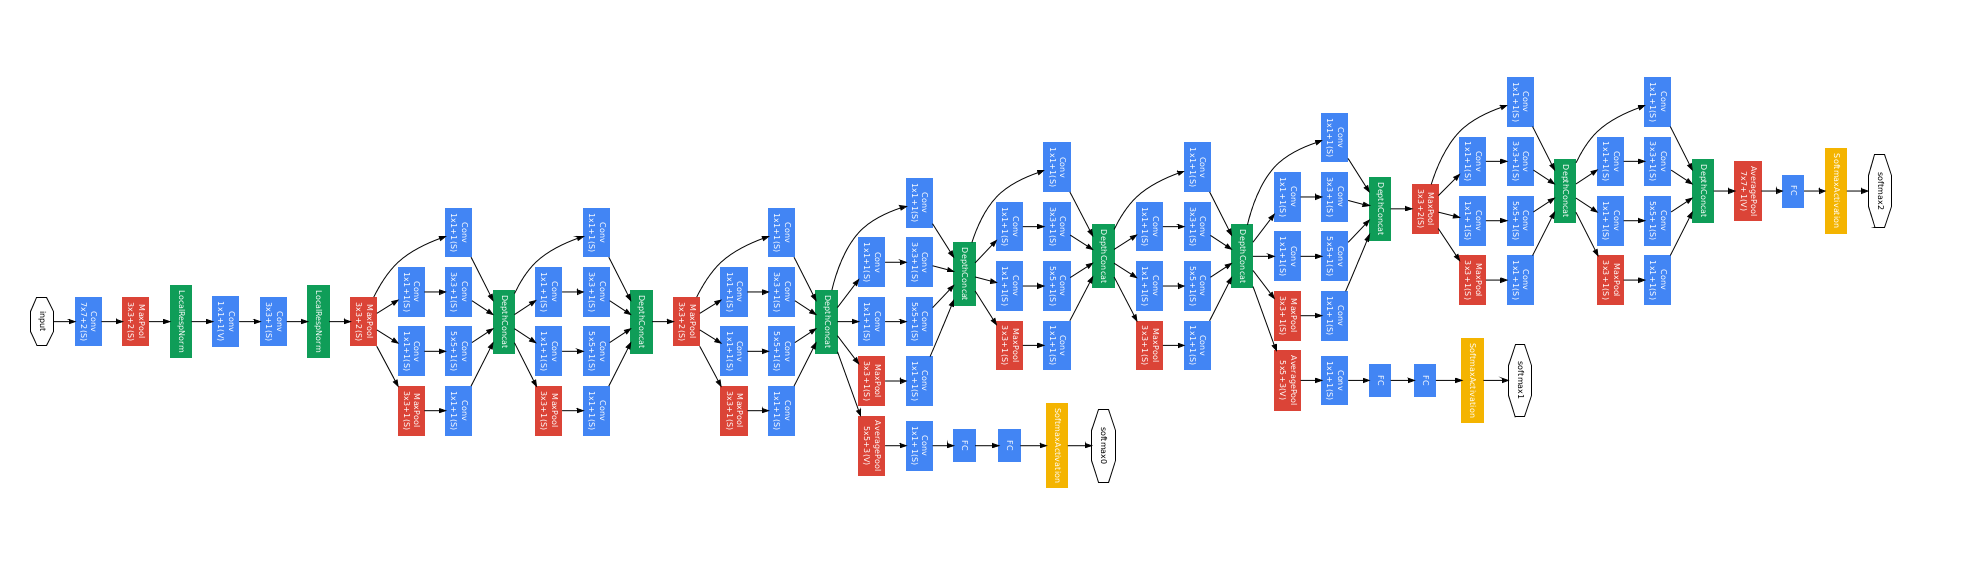
\includegraphics[width=\textwidth]{img/googlenet_diagram.png}
\end{center}

\end{frame}

%%%%%%%%%%%%%%%%%%%%%%%%%%%%%%%%%%%%%%%%%%%%%%%%%%%
\begin{frame}[fragile] \frametitle{} \oldB \small

\textbf{\magenta{Python demo V: GoogLeNet - Inception Module}}

\end{frame}

%%%%%%%%%%%%%%%%%%%%%%%%%%%%%%%%%%%%%%%%%%%%%%%%%%%
\begin{frame}[fragile] \frametitle{} \oldB \small

\yblue{\textbf{Batch Normalization (2015)}}

Not a model architecture itself, but one very useful new tweak in
the past year has been Batch Normalization, first presented in this
paper:
\begin{quote}
 Ioffe, Sergey, and Christian Szegedy. "Batch normalization: Accelerating deep network training by reducing internal covariate shift." arXiv preprint arXiv:1502.03167
\end{quote}

\end{frame}

%%%%%%%%%%%%%%%%%%%%%%%%%%%%%%%%%%%%%%%%%%%%%%%%%%%
\begin{frame}[fragile] \frametitle{} \oldB \small

\textbf{\magenta{Python demo VI: Batch normalization}}

\end{frame}

%%%%%%%%%%%%%%%%%%%%%%%%%%%%%%%%%%%%%%%%%%%%%%%%%%%
\begin{frame}[fragile] \frametitle{} \oldB \small

\yblue{\textbf{PReLUnet (2015)}}

Microsoft's first contribution in 2015 was the idea of using
a modifed ReLU activation function:
\begin{quote}
He, Kaiming, et al. "Delving deep into rectifiers: Surpassing human-level performance on imagenet classification." Proceedings of the IEEE International Conference on Computer Vision. 2015.
\end{quote}

\end{frame}

%%%%%%%%%%%%%%%%%%%%%%%%%%%%%%%%%%%%%%%%%%%%%%%%%%%
\begin{frame}[fragile] \frametitle{} \oldB \small

\begin{center}
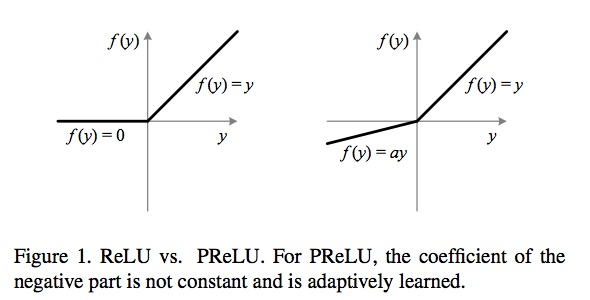
\includegraphics[width=\textwidth]{img/prelunetActivation.jpg}
\end{center}

\end{frame}

%%%%%%%%%%%%%%%%%%%%%%%%%%%%%%%%%%%%%%%%%%%%%%%%%%%
\begin{frame}[fragile] \frametitle{} \oldB \small

\yblue{\textbf{ResNet-50, -101, -152 (2015)}}

Finally, in the 2015 competition, Microsoft produced an model
which is extremely deeper than any previously used. These models
are known as ResNet, with their depth given as an suffix.
\begin{quote}
He, Kaiming, Xiangyu Zhang, Shaoqing Ren, and Jian Sun.
"Deep Residual Learning for Image Recognition." arXiv preprint
arXiv:1512.03385 (2015).
\end{quote}

\end{frame}

%%%%%%%%%%%%%%%%%%%%%%%%%%%%%%%%%%%%%%%%%%%%%%%%%%%
\begin{frame}[fragile] \frametitle{} \oldB \small

\begin{center}
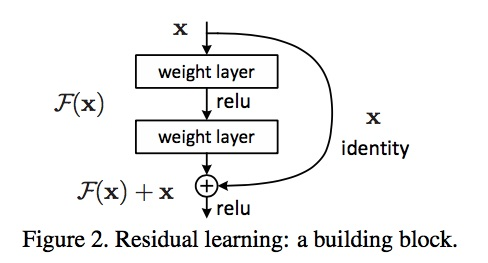
\includegraphics[width=\textwidth]{img/resNetresidualUnit.jpg}
\end{center}

\end{frame}


%%%%%%%%%%%%%%%%%%%%%%%%%%%%%%%%%%%%%%%%%%%%%%%%%%%
\begin{frame}[fragile] \frametitle{} \oldB \small

\begin{center}
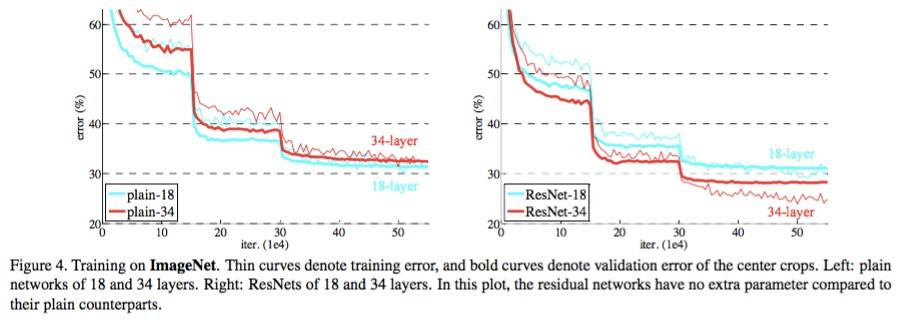
\includegraphics[width=\textwidth]{img/resNetPerform.jpg}
\end{center}

\end{frame}


%%%%%%%%%%%%%%%%%%%%%%%%%%%%%%%%%%%%%%%%%%%%%%%%%%%
\begin{frame}[fragile] \frametitle{} \oldB \small

\begin{center}
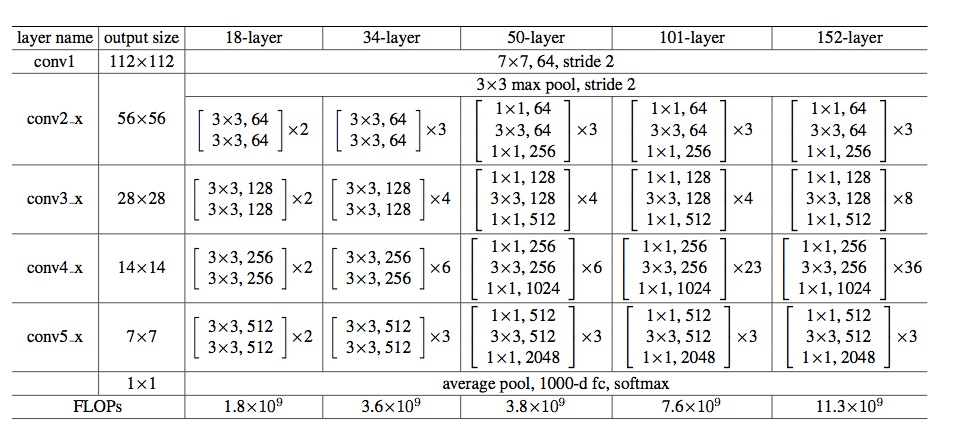
\includegraphics[width=\textwidth]{img/resNetModel.jpg}
\end{center}

\end{frame}

%%%%%%%%%%%%%%%%%%%%%%%%%%%%%%%%%%%%%%%%%%%%%%%%%%%
\begin{frame}[fragile] \frametitle{} \oldB \small

\begin{center}
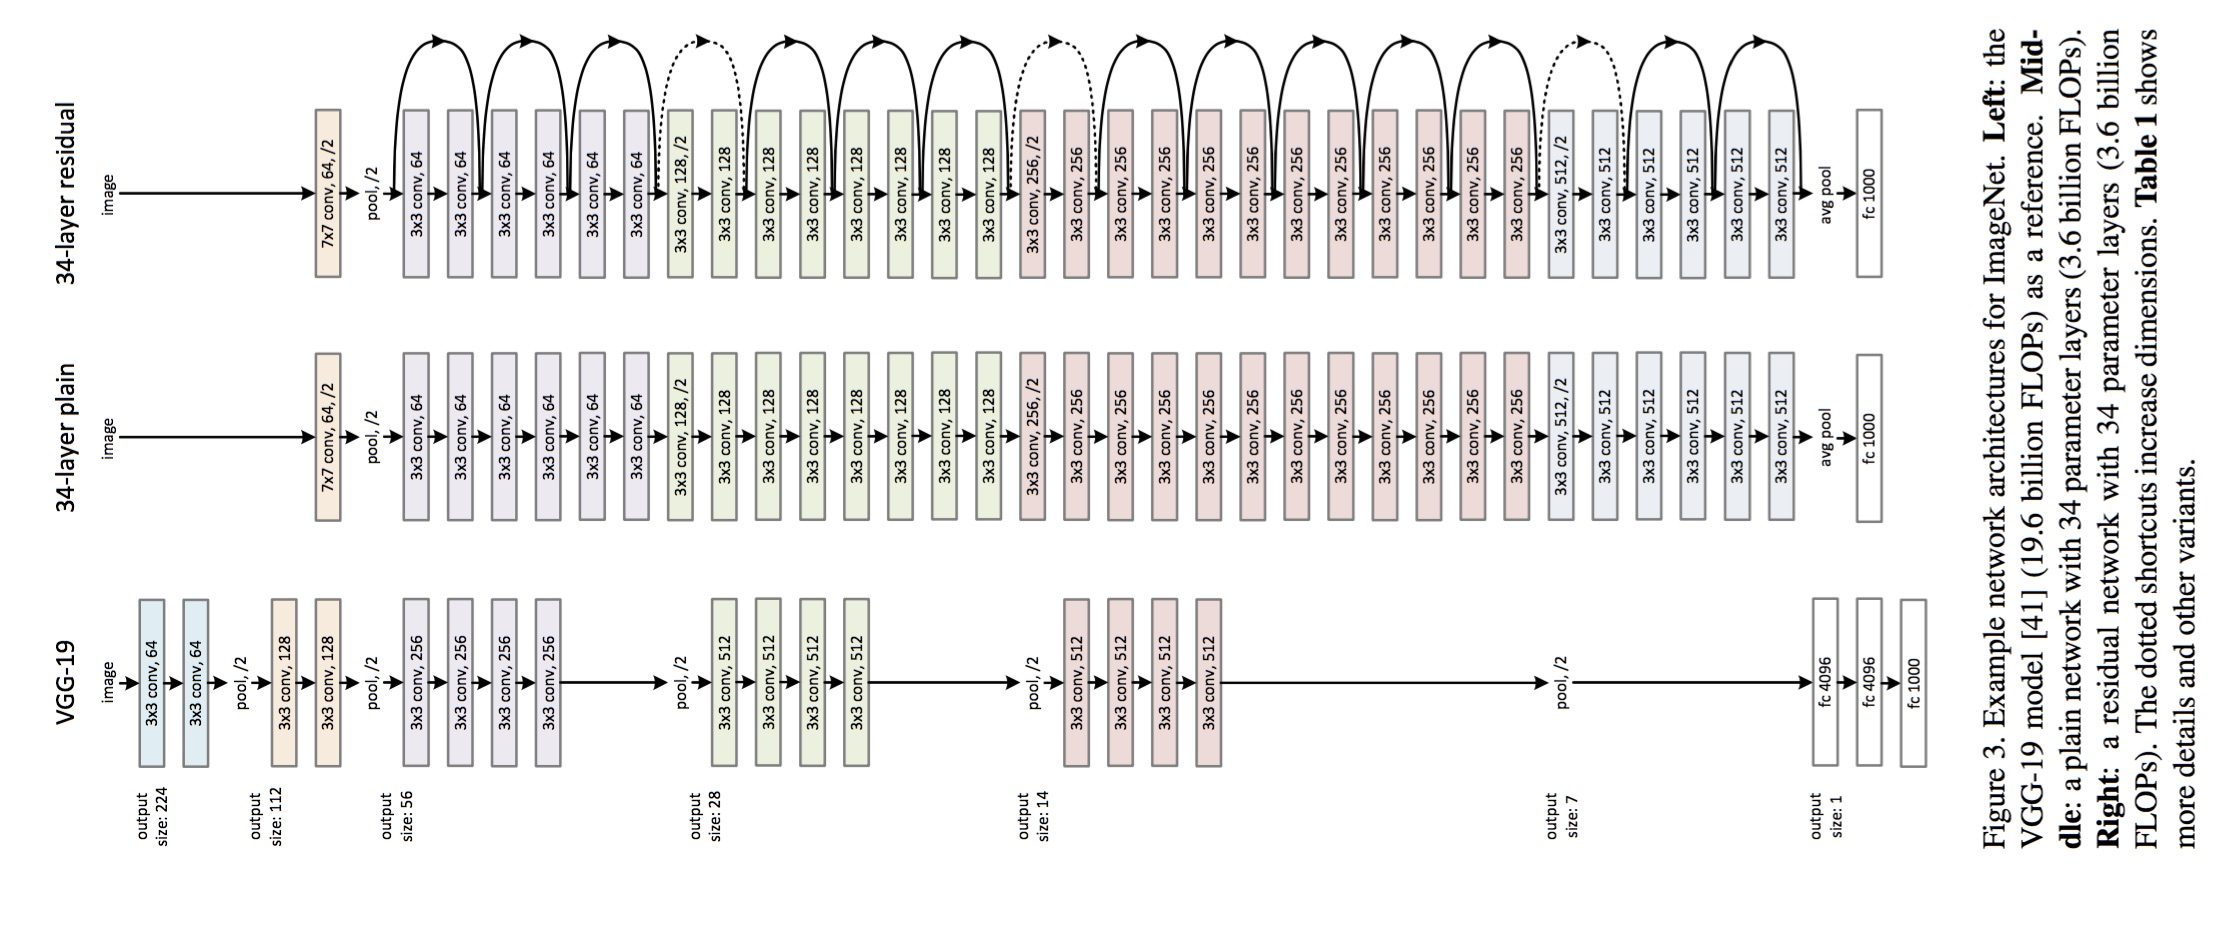
\includegraphics[width=\textwidth]{img/resNet.jpg}
\end{center}

\end{frame}


%%%%%%%%%%%%%%%%%%%%%%%%%%%%%%%%%%%%%%%%%%%%%%%%%%%
\begin{frame}[fragile] \frametitle{} \oldB \small

\yblue{\textbf{Stochastic Depth Models (2016)}}

Another tweak on the ResNet architecture, which subsamples
layers in the network:
\begin{quote}
Gao Huang, Yu Sun, Zhuang Liu, Daniel Sedra, Kilian Weinberger.
"Deep Networks with Stochastic Depth", arXiv preprint arXiv:1603.09382 (2016).
\end{quote}
Notice how this seems like an almost obvious thing to try
given the ResNet architecture, but less-so in a generic
neural network.

\end{frame}

%%%%%%%%%%%%%%%%%%%%%%%%%%%%%%%%%%%%%%%%%%%%%%%%%%%
\begin{frame}[fragile] \frametitle{} \oldB \small

\begin{center}
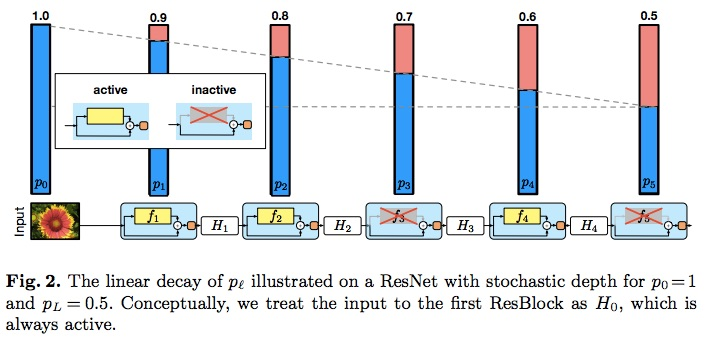
\includegraphics[width=0.8\textwidth]{img/sampleNet.jpg}
\end{center}

\end{frame}

%%%%%%%%%%%%%%%%%%%%%%%%%%%%%%%%%%%%%%%%%%%%%%%%%%%
\begin{frame}[fragile] \frametitle{} \oldB \small

\yblue{\textbf{ResNet-200, -1001 (2016)}}

Microsoft's update to last year's model. Posted only two
weeks ago!
\begin{quote}
He, Kaiming, et al. "Identity Mappings in Deep Residual Networks." arXiv preprint arXiv:1603.05027 (2016).
\end{quote}

\end{frame}

%%%%%%%%%%%%%%%%%%%%%%%%%%%%%%%%%%%%%%%%%%%%%%%%%%%
\begin{frame}[fragile] \frametitle{} \oldB \small

\begin{center}
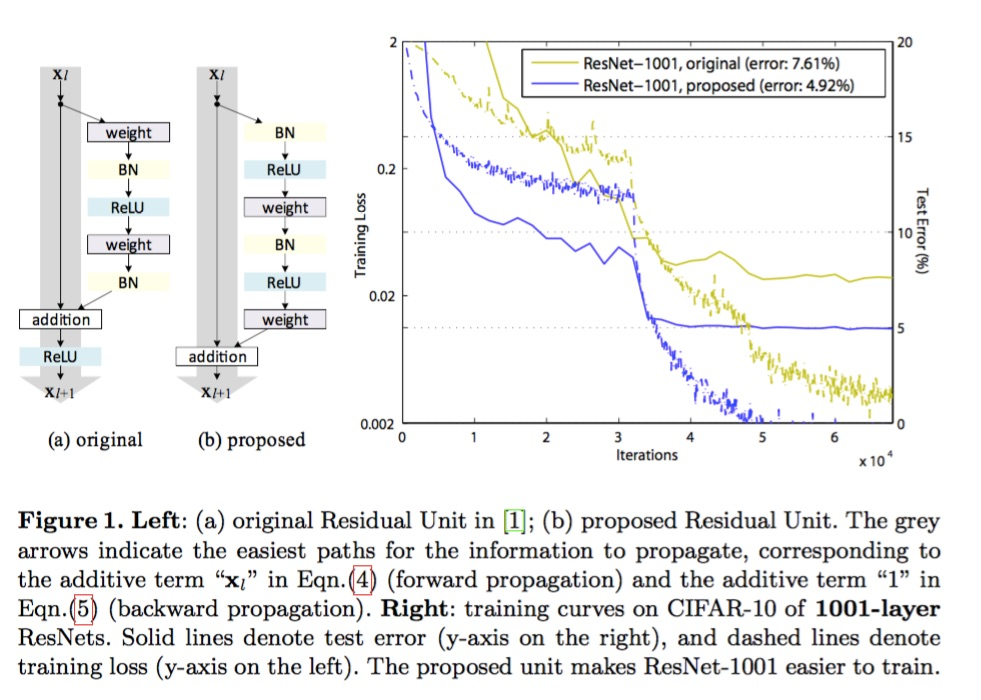
\includegraphics[width=0.8\textwidth]{img/resNet1001.jpg}
\end{center}

\end{frame}

%%%%%%%%%%%%%%%%%%%%%%%%%%%%%%%%%%%%%%%%%%%%%%%%%%%
\begin{frame}[fragile] \frametitle{} \oldB \small

\yblue{\textbf{SqueezeNet (2016)}}

A new line of research involves looking at ways to produce near
state-of-the-art results with a minimal model size (or minimal
computational cost):
\begin{quote}
Iandola, Forrest N., et al. "SqueezeNet: AlexNet-level accuracy with
50x fewer parameters and <1MB model size." arXiv preprint arXiv:1602.07360 (2016).
\end{quote}

\end{frame}

%%%%%%%%%%%%%%%%%%%%%%%%%%%%%%%%%%%%%%%%%%%%%%%%%%%
\begin{frame}[fragile] \frametitle{} \oldB \small

\begin{center}
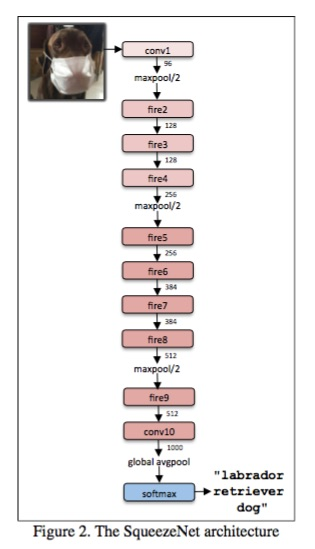
\includegraphics[width=0.3\textwidth]{img/squeezeNetModel.jpg}
\end{center}

\end{frame}

%%%%%%%%%%%%%%%%%%%%%%%%%%%%%%%%%%%%%%%%%%%%%%%%%%%
\begin{frame}[fragile] \frametitle{} \oldB \small

\begin{center}
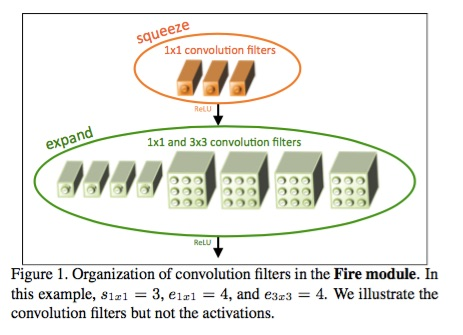
\includegraphics[width=0.7\textwidth]{img/squeezeNetFire.jpg}
\end{center}

\end{frame}

%%%%%%%%%%%%%%%%%%%%%%%%%%%%%%%%%%%%%%%%%%%%%%%%%%%
\begin{frame}[fragile] \frametitle{} \oldB \small

\begin{center}
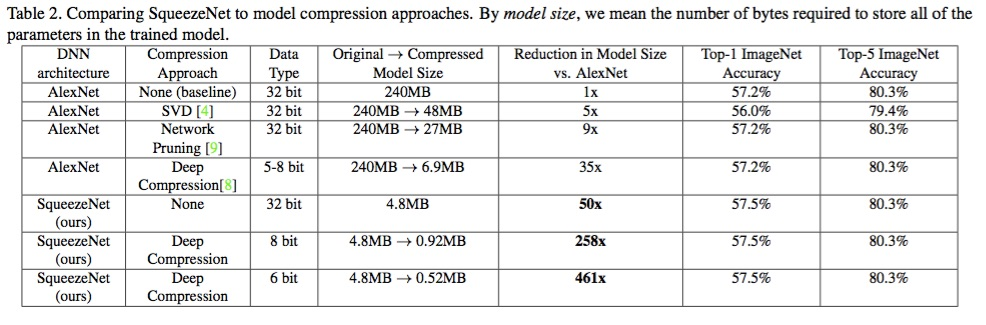
\includegraphics[width=\textwidth]{img/squeezeNetResults.jpg}
\end{center}

\end{frame}

%%%%%%%%%%%%%%%%%%%%%%%%%%%%%%%%%%%%%%%%%%%%%%%%%%%
\begin{frame}[fragile] \frametitle{} \oldB \small

\textbf{\yblue{Microsoft Common Images in Context (MS COCO)}}

\begin{center}
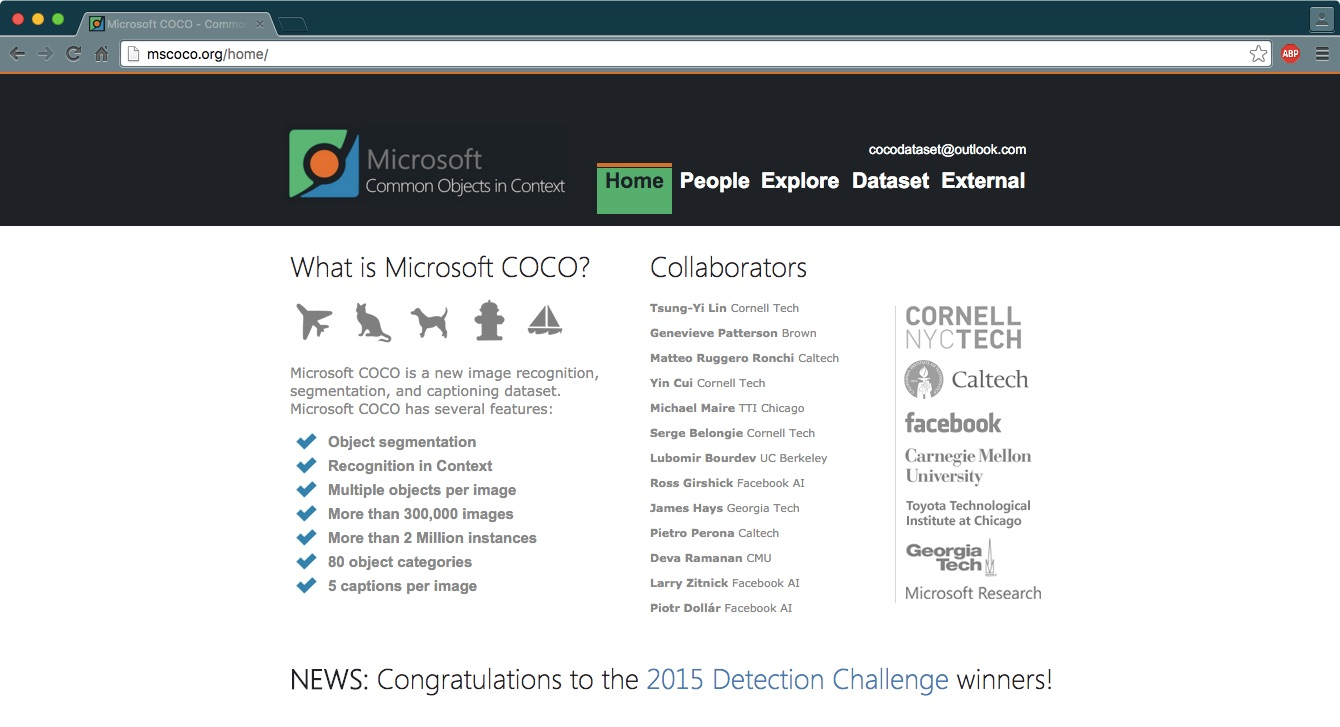
\includegraphics[width=\textwidth]{img/mscocoWeb.jpg}
\end{center}

\end{frame}

%%%%%%%%%%%%%%%%%%%%%%%%%%%%%%%%%%%%%%%%%%%%%%%%%%%
\begin{frame}[fragile] \frametitle{} \oldB \small

\begin{center}
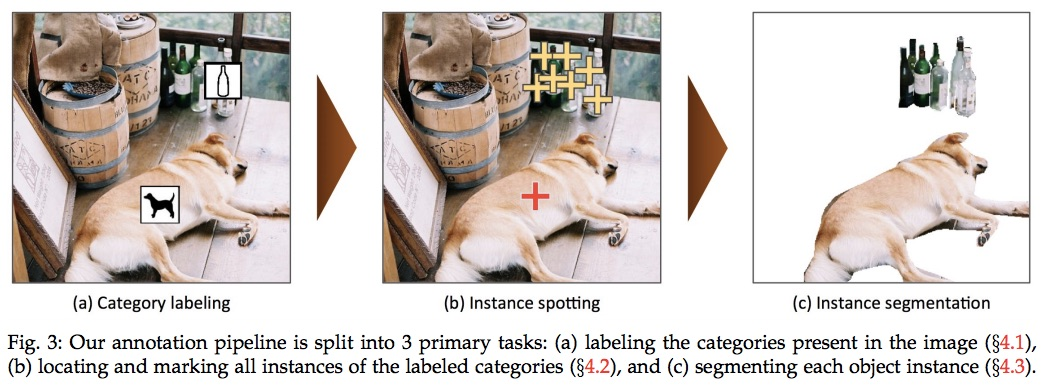
\includegraphics[width=\textwidth]{img/segmentMSCOCO.jpg}
\end{center}

\end{frame}

%%%%%%%%%%%%%%%%%%%%%%%%%%%%%%%%%%%%%%%%%%%%%%%%%%%
\begin{frame}[fragile] \frametitle{} \oldB \small

\begin{center}
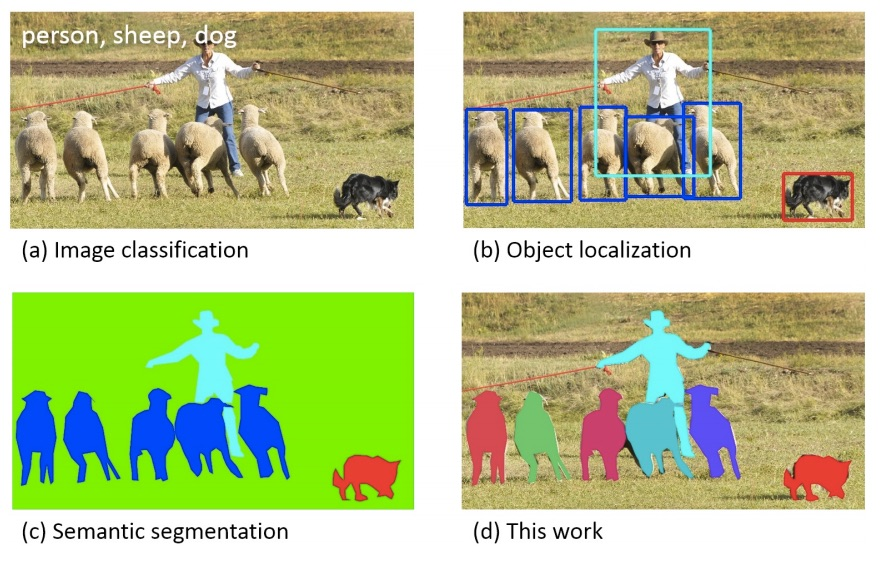
\includegraphics[width=0.75\textwidth]{img/segmentMSCOCO2.jpg}
\end{center}

\end{frame}

%%%%%%%%%%%%%%%%%%%%%%%%%%%%%%%%%%%%%%%%%%%%%%%%%%%
\begin{frame}[fragile] \frametitle{} \oldB \small

More information is found on their website, \url{http://mscoco.org/},
and in the paper describing the dataset:
\begin{quote}
Lin, Tsung-Yi, et al. "Microsoft coco: Common objects in context."
Computer Vision–ECCV 2014. Springer International Publishing, 2014. 740-755.
\end{quote}

\end{frame}



\end{document}







